% Chapter 3

\chapter{Background} % Main chapter title

\label{Chapter3} % For referencing the chapter elsewhere, use \ref{Chapter3} 

We present a brief history of memory attacks and some background information on
control-flow attacks in Section~\ref{sec:control-flow-attack}. In
Section~\ref{sec:remote-attestation}, we discuss how remote attestation helps to
detect control-flow attack. We present ScaRR control flow model in
Section~\ref{sec:scarr-model}. We present an overview of LLVM that is relevant
to the research in Section~\ref{sec:llvm}.

\section{Control Flow Attack}
\label{sec:control-flow-attack}

A control-flow attack happens when an adversary maliciously makes a program act
on his choice. The adversary can do so without statically modifies the program
binary but alters the runtime properties of the program. The adversary intention
can be to execute malicious operations or to leak secret information. Many of
these runtime software security attacks occur due to memory corruption bug
in software written in low-level languages like C and
C++~\cite{szekeresSoKEternalWar2013}.

Once memory corruption is triggered, there are different exploit types which
adversary can use to perform the attack. Some of the relevant exploits are
control-flow hijack~\cite{shachamGeometryInnocentFlesh2007,
schusterCounterfeitObjectorientedProgramming2015}  and data only
attack~\cite{chenNonControlDataAttacksAre2005,
carliniControlFlowBendingEffectiveness2015}. 

We can classify control-flow hijack into code injection attacks and code reuse
attacks. Code injection attack injects malicious codes to the program. The
malicious code executes action prepared by the attacker. We can mitigate code
injection attacks using solutions like non-executable stack (NX), Data Execution
Prevention and \( W \bigoplus R \)~\cite{vanderveenMemoryErrorsPresent2012}.
Code reuse attack executes malicious action without injecting any codes. Return
oriented programming~\cite{roemerReturnorientedProgrammingSystems2012} is
example of code reuse attack. Return-oriented program chains together short
instruction sequences already present in the program. Specifically, adversaries
use instruction that ends in a \texttt{return} opcode. Unfortunately, ROP cannot
be mitigated by \( W \bigoplus R
\)~\cite{roemerReturnorientedProgrammingSystems2012}.

Memory error attacks and defenses are a continuous battle which unfortunately
has not shown that it is over. In 2016, Abera et al proposed to use remote
attestation to detect control flow
attack~\cite{aberaCFLATControlFlowAttestation2016}. That paper opened many types
of research in this area which we briefly presented in Chapter~\ref{Chapter1}.
 
\section{Remote Attestation}
\label{sec:remote-attestation}

In this thesis, we explore the use of remote attestation in detecting the
control-flow attack. The goal of remote attestation is to validate the state of
a remote system. Generally, we implement the remote attestation as protocol with
two parties, the verifier as the attester and the remote system as the prover.
Prover provides evidence to verifier over a
network~\cite{cokerPrinciplesRemoteAttestation2011a}. The ubiquitous deployment
of IoT and different applications in the cloud require a robust remote
attestation method. A good remote attestation can ensure the detection of any
attacks. Initially, remote attestation only covers static attestation of the
application binary. However, in recent years there has been a more sophisticated
attack that can alter application behaviors; so that only static attestation
does not suffice. 

As we mention above, there are two roles involved in the remote attestation.
They are a trusted prover and a verifier. A prover is the one that must prove
that the software runtime integrity. Verifier checks prover to ask the current
state of the runtime of the program. Alternatively, the prover also can update
the verifier periodically without an explicit trigger from the verifier. The
verifier checks the prover response with the local database. If any of
measurement mismatches, it means the has been a violation due to the attacks.

This research mainly focuses on offline measurement data generation for remote
attestation. The verifier uses the offline measurement in the local database to
validate the control-flow graph.  We discuss the detail of the control-flow
model in Section~\ref{sec:scarr-model}. We write the offline program analyzer
using LLVM. We discuss some LLVM backgrounds in Section~\ref{sec:llvm}.

\section{ScaRR Control-Flow Model} 
\label{sec:scarr-model}

ScaRR~\cite{toffaliniScaRRScalableRuntime2019} takes lesson learned from many
former runtime remote attestation scheme to build a model that can perform in a
scalable way and can perform remote attestation on a complex system. ScaRR
control-flow model consists of two main components, checkpoint and list of
action. 

As with many previous runtime attestation schemes, ScaRR models and validates
the attestation based on the program's control flow graph. We need to run
one-time measurement computation to extract checkpoints and list of actions of
the program.

\subsection{Checkpoints} \label{sec:scarr-checkpoints} Checkpoint is basic block
of the program that delimits the execution path of the program. ScaRR defines
these different checkpoint types:
\begin{itemize}
    \item Thread Beginning: demarcating the start of program/thread
    \item Thread End: demarcating the end of program/thread
    \item Exit Point: representing exit point from an application such as system
    call or out of translation unit function/library call
    \item Virtual-Checkpoint: managing cases for loop or recursion
\end{itemize}

In a program, there should be at least Thread Beginning and Thread End
checkpoints. Later, depends on the structure of the program, some different
checkpoints are marked in the program CFG.

\subsection{List of Actions}

List of actions (LoA) are edges (marked by two checkpoints) that direct one
checkpoint to the next one. In a program execution path, we only consider edges
that identify the unique execution path.

LoA is defined through the following notation:


$$[(BBL_{s1},BBL_{d1}),...,(BBL_{sn},BBL_{dn})]$$

Consider again the CFG in the Figure~\ref{fig:simple-loop-checkpoints}. The LoA
between $N_3$ (Checkpoint Virtual) and $N_{10}$ (checkpoint ThreadEnd) is
$[(BBL_3, BBL_{10})]$. However, the LoA between $N_0$ and $N_3$ is $[]$ (empty
set).

\begin{figure}[htbp]
    \centerline{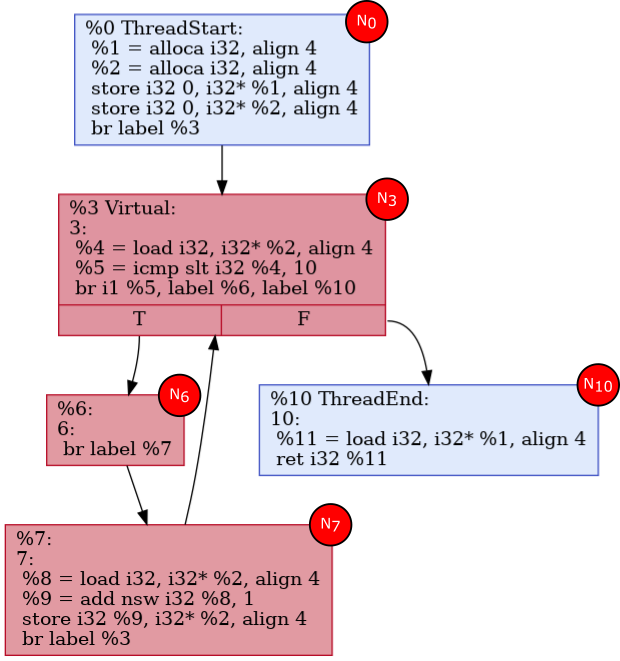
\includegraphics[scale=.70]{Figures/03/simple-loop-checkpoints.png}}
    \caption{Loop CFG.}
    \label{fig:simple-loop-checkpoints}
\end{figure}


\section{LLVM}
\label{sec:llvm}

LLVM is a compiler framework developed by Chris Lattner. LLVM provides portable
program representation and different compiler toolings. LLVM supports the
implementation of various frontends, backends, and middle optimizers for many
programming languages~\cite{lattnerLLVMCompilationFramework2004a}. 

\subsection{Intermediate Representation}

LLVM intermediate representation (IR) is a high-level representation of programs
that enables analysis, instrumentations, and transformations. However, the IR is
sufficiently low-level to represent arbitrary programs and to allow broad
optimization. 


\begin{listing}[htbp]
    \inputminted[
    frame=lines,
    framesep=2mm,
    baselinestretch=1.2,
    fontsize=\footnotesize,
    linenos
    ]{c}{Code/03/sample.c}
    \caption{Simple C Program.}    
    \label{listing:sample-c}
\end{listing}

Listing~\ref{listing:sample-c} show a simple C program. The IR of the code in
Listing~\ref{listing:sample-c} is in Listing~\ref{listing:sample-ll}. The text
representation is just one form of IR. Besides this readable instruction
representation, LLVM IR also can be represented as byte code and in-memory
representation. In the IR, each line contains LLVM instructions. We group
instructions into basic blocks: containers for instructions that execute
sequentially. This arrangement explicitly represent application control-flow
graph (CFG) in the IR. The details of LLVM IR is available in the Language
Reference~\cite{LLVMLanguageReferencea}.

\begin{listing}[ht]
    \inputminted[
    frame=lines,
    framesep=2mm,
    baselinestretch=1.2,
    fontsize=\footnotesize,
    linenos
    ]{llvm}{Code/03/sample.ll}
    \caption{LLVM IR The Sample C Program.}    
    \label{listing:sample-ll}
\end{listing}


\begin{figure}[ht]
    \centerline{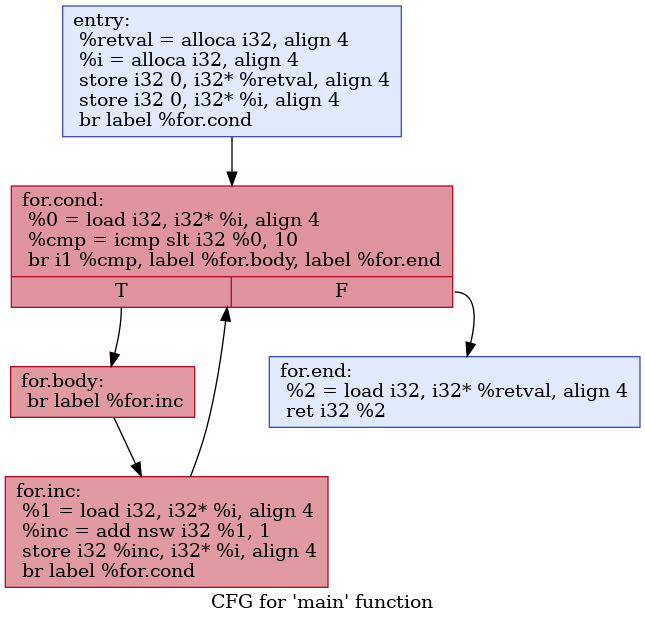
\includegraphics[scale=.75]{Figures/03/cfg.png}}
    \caption{CFG for Simple C Program.}
    \label{fig:cfg}
\end{figure}


LLVM optimizer --- which includes Analyzer and Transformer --- are working on
IR. In this thesis, we are using this analyzer and transformer in building the
Offline Program Analyzer.

\begin{figure}[htbp] 
    \centerline{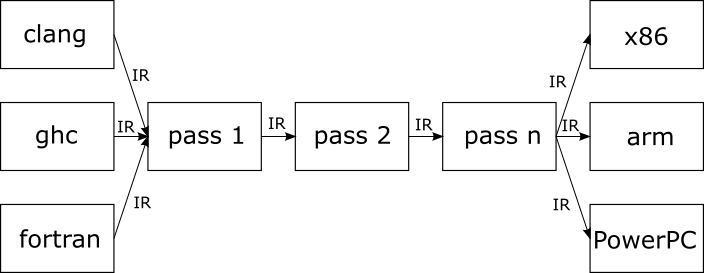
\includegraphics[scale=.75]{Figures/03/llvm-overview.png}} 
    \caption{LLVM Pass.} 
    \label{fig:llvm} 
\end{figure} 

\subsection{LLVM Pass}

LLVM applies transformations --- which may include some analysis pipelines ---
and optimizations on tools called \texttt{opt}. \texttt{opt} is taking LLVM IR
(either as text, bytecode or in memory) as input and then do transformations,
analysis, and optimizations on it (see Figure~\ref{fig:llvm}). Transformation
and optimization alter the LLVM structure. The analysis gets information from
the structure, which usually to be used by one or more transformations. LLVM
performs different transformations, optimizations, and analyses as pipelines of
passes. LLVM pass can run per function, module or loop. LLVM executes function
pass once for every function in the program. LLVM module pass is executed once
for every module. LLVM loop pass runs a time for each loop.  


In LLVM, there are two ways of implementing pass. First, to use the legacy
approach. The latest one, to use the new pass manager approach. The approach is
different (1) in structuring the code for the pass and also (2) the way we use
the pass. In the legacy approach, we need to inherit from either
\texttt{ModulePass}, \texttt{FunctionPass} or \texttt{LoopPass} and override
\texttt{runOnXXX} method (xxx is either Function, Module, or Loop). In the newer
approach, we have to inherit CRTP mix-in \texttt{PassInfoMixin<PassT>} and
override the run method.

In the legacy approach, we need to provide the pass name as a literal argument
to \texttt{opt}. See the example in Listing~\ref{listing:legacy-llvm-pass}. In
the new pass manager, we are putting the pass name after \texttt{--passes}
argument in comma-separated list (Listing~\ref{listing:new-llvm-pass}). LLVM
executes the passes in order.

\begin{listing}[htbp]
    \begin{minted}[
        frame=lines,
        framesep=2mm,
        baselinestretch=1.2,
        fontsize=\footnotesize,
        ]{bash}
        opt --dot-cfg file.ll 
    \end{minted}
    \caption{Running Legacy LLVM Pass.}    
    \label{listing:legacy-llvm-pass}
\end{listing}

\begin{listing}[htpb]
    \begin{minted}[
        frame=lines,
        framesep=2mm,
        baselinestretch=1.2,
        fontsize=\footnotesize,
        ]{bash}
        opt -passes=scarr-cp-marker,scarr-loa-collector file.ll 
    \end{minted}
    \caption{Running LLVM New Pass.}    
    \label{listing:new-llvm-pass}
\end{listing}

\subsection{LLVM API}

In writing the LLVM pass, we use LLVM API. In this section, we present relevant
component that is required in implementing LLVM Pass for the Offline Program
Analyzer. LLVM API is leveraging many C++ features and libraries such as
template and STL. The API also provides many ready to use data structure which
is not available in the STL. A more broad discussion on the important elements
of the API is available in the Programmers Manual~\cite{LLVMProgrammerManuala}.
We also can refer to the Complete API documentation in the doxygen
page~\cite{LLVMLLVMa}.

\subsubsection{Module}

Module is the top-level container for all other IR objects. Module contains a
list of global variables, functions, symbol tables, and other various data about
target characteristics. Module can present as a single translation unit of a
program (source file) or can be multiple translation units combined by a linker.


In LLVM pass, we can get access to a module by implementing a texttt{Module}
pass or by parsing IR using \texttt{parseIR} or \texttt{parseIRFile} from
\texttt{IRReader.h}. Once we get a handler to a module, getting a functions
within module is as simple as pass a module to a loop.  Module provides iterator
that returns list of functions in the module (see
Listing~\ref{listing:llvm-module-api}).

\begin{listing}[htbp]
    \inputminted[
        frame=lines,
        framesep=2mm,
        baselinestretch=1.2,
        fontsize=\footnotesize,
        linenos
    ]{cpp}{Code/03/module.cpp}
    \caption{LLVM Module API.}    
    \label{listing:llvm-module-api}
\end{listing}

\subsubsection{Function}

Function in LLVM represents a function in the source program. A function
contains a list of zero or more BasicBlocks. There is one entry BasicBlock and
can be multiple exit BasicBlocks. We can get a handler to a function either by
getting the iterator from a module instance or by implementing a Function Pass.
By using optimization, syntax hint, or using an inliner pass, a function can be
inlined. In this thesis, we are using \emph{inliner-wrapper} pass to inline most
functions before feeding the IR into the ScaRR passes. See also
Section~\ref{sec:code-inlining} which discusses the inlining process.

\subsubsection{Basic Block}

Basic Block represents a single entry and single exit section of the code. The
single exit can be one of terminator instruction -- branches, return, unwind and
invoke. We can get a handle to a basic block from function. Refer to
Listing~\ref{listing:llvm-basic-block-api} to see how to get the basic block.

\begin{listing}[htbp]
    \begin{minted}[
        frame=lines,
        framesep=2mm,
        baselinestretch=1.2,
        fontsize=\footnotesize,
        linenos
    ]{cpp}
        for (auto &function: *module) {
            for (auto &basicBlok: function) {
                // do thing with Basic Block
            }
        }
    \end{minted}
    \caption{LLVM Basic Block API.}    
    \label{listing:llvm-basic-block-api}
\end{listing}

\subsubsection{Graph Traversal}

LLVM CFG is structured as a graph. Therefore the basic block can be traversed
using different ready-to-use graph traversal algorithms. LLVM offers some common
graph traversal algorithms such as breadth-first search and depth-first search.
The algorithms can be used immediately on basic blocks and functions. If there
is a need to traverse a custom structure, the algorithms just require the new
structure to implement \emph{GraphWriter} interface.

\subsection{Tools}

We are implementing the algorithms using different tools. We are highlighting
some of those in this section so that everyone interested can replicate the
step.

\subsubsection{clang}

\texttt{clang} is one of the frontend provided by LLVM. It can compiles C, C++
and Objective C. \texttt{clang} command-line arguments are compatible with
widely use GCC compiler. The main use of \texttt{clang} in this research is to
compile source files into LLVM IR text files.
Listing~\ref{listing:compile-llvm-to-ir} shows how to compile a C program into
LLVM IR. 

\begin{listing}[htbp]
    \begin{minted}[
        frame=lines,
        framesep=2mm,
        baselinestretch=1.2,
        fontsize=\footnotesize,
    ]{bash}
        clang -S -emit-llvm source.c
    \end{minted}
    \caption{Compiling C to LLVM IR.}    
    \label{listing:compile-llvm-to-ir}
\end{listing}
    
We can pass the optimization level from 0 (no optimization) to 3 (maximum
optimization) when compiling the source code. The optimization level 3 makes
code run faster but it produces a larger code size.

By default, clang strips out value names and optimizes the code when generating
LLVM IR. We can use this flag to disable optimization and get readable value
names that can help when troubleshooting and exploring the generated IR.
Listing~\ref{listing:compile-llvm-to-ir-no-opt} shows how to compile to IR
without any optimization and to preserve the function and variable names.

\begin{listing}[htbp]
    \begin{minted}[
        frame=lines,
        framesep=2mm,
        baselinestretch=1.2,
        fontsize=\footnotesize,
    ]{bash}
        clang -S -emit-llvm -Xclang -disable-O0-optnone \
        -fno-discard-value-names source.c
    \end{minted}
    \caption{Compiling C to LLVM IR without Optimization.}    
    \label{listing:compile-llvm-to-ir-no-opt}
\end{listing}

\subsubsection{opt}

\texttt{opt} is the LLVM optimizer and analyzer that can be invoked from the
command line. We use \texttt{opt} to execute the offline program analyzer which
marks basic block checkpoints and calculate list of actions which can be used as
information to detect control flow violations during remote attestation.

\subsubsection{cmake}

\texttt{cmake} is a build file generator that has an important role in large
projects like LLVM. Although a deep understanding of \texttt{cmake} is not
required in implementing LLVM pass, but we need to know at least how to build
the pass after the implementation so that we can run it.

We can download LLVM uses git. See Listing~\ref{listing:clone-llvm-code}. We
implement the offline measurement extract using LLVM 13.0.0.

\begin{listing}[htbp]
    \begin{minted}[
        frame=lines,
        framesep=2mm,
        baselinestretch=1.2,
        fontsize=\footnotesize,
    ]{bash}
        git clone https://github.com/llvm/llvm-project
    \end{minted}
    \caption{Cloning LLVM Source Code.}    
    \label{listing:clone-llvm-code}
\end{listing}

After downloading the code, we can go to the LLVM directory and generate the
build files. \texttt{cmake} supports several build tools such as make and ninja.
Refer to Listing~\ref{listing:build-llvm}.

\begin{listing}[htbp]
    \begin{minted}[
        frame=lines,
        framesep=2mm,
        baselinestretch=1.2,
        fontsize=\footnotesize,
        linenos
    ]{bash}
        cd llvm-project/llvm
        mkdir build
        cd build
        cmake -G Ninja ../ # generate build file for Ninja
        ninja opt # build only opt
    \end{minted}
    \caption{Building LLVM.}    
    \label{listing:build-llvm}
\end{listing}

With all background discussion in this chapter, we should be ready to discuss
the methodology in Chapter~\ref{Chapter4}.